% Mathlib Cocycle Splitting Companion — Technical note for Mathlib reviewers.
% Companion technical note for the Mathlib PR (Paper B).
\documentclass[11pt]{article}
\input{../suite_preamble}
\usepackage{longtable}
\usepackage{listings}
\usepackage{tikz}
\usetikzlibrary{arrows.meta, positioning, calc}
\lstdefinelanguage{lean}{
  keywords={def, noncomputable, theorem, lemma, structure, class, instance, where, by,
            exact, rfl, simp, intro, have, let, refine, rcases, obtain, cases, fun,
            apply, rw, show, calc, import, open, variable, namespace, end, section,
            private, abbrev, attribute, set, conv_rhs},
  keywordstyle=\bfseries,
  ndkeywords={Prop, Type, Sort, Nat, Group, CommGroup, MulAut, Nonempty, MonoidHom,
              Subgroup, Subtype, Function, GroupExtension, Section, Splitting},
  ndkeywordstyle=\bfseries,
  sensitive=true,
  comment=[l]{--},
  morecomment=[s]{/-}{-/},
  commentstyle=\itshape,
  stringstyle=\ttfamily,
  basicstyle=\ttfamily\small,
  breaklines=true,
  showstringspaces=false,
  columns=flexible
}
\lstset{language=lean,
  literate=
    {₁}{{$_1$}}1 {₂}{{$_2$}}1 {₃}{{$_3$}}1
    {⁻¹}{{$^{-1}$}}1
    {→}{{$\to$}}1 {←}{{$\leftarrow$}}1
    {⟶}{{$\longrightarrow$}}1 {⟵}{{$\longleftarrow$}}1
    {⥤}{{$\Rightarrow$}}1
    {≫}{{$\gg$}}1
    {∀}{{$\forall$}}1 {∃}{{$\exists$}}1
    {⟨}{{$\langle$}}1 {⟩}{{$\rangle$}}1
    {≤}{{$\le$}}1 {≥}{{$\ge$}}1 {≠}{{$\ne$}}1
    {∈}{{$\in$}}1 {∉}{{$\notin$}}1
    {ℕ}{{$\mathbb{N}$}}1 {ℤ}{{$\mathbb{Z}$}}1
    {⊗}{{$\otimes$}}1 {⊕}{{$\oplus$}}1
    {≃}{{$\simeq$}}1
    {∘}{{$\circ$}}1
    {·}{{$\cdot$}}1
    {↔}{{$\leftrightarrow$}}1
    {¹}{{$^1$}}1 {²}{{$^2$}}1
    {σ}{{$\sigma$}}1
    {φ}{{$\varphi$}}1
    {η}{{$\eta$}}1
    {α}{{$\alpha$}}1
    {β}{{$\beta$}}1
    {ε}{{$\varepsilon$}}1
    {π}{{$\pi$}}1
    {τ}{{$\tau$}}1
    {ψ}{{$\psi$}}1
    {Σ}{{$\Sigma$}}1
}
\input{../suite_macros}

\title{Completing the Cohomological Extension Package:\\[0.35em]
\large Section Cocycles and Splitting Criteria for Mathlib}
\author{Nova Spivack}
\date{2026}

\begin{document}

\maketitle

\begin{abstract}
Mathlib's \texttt{GroupExtension/Defs.lean} documents two explicit TODO items:
a bijection between $N$-conjugacy classes of splittings and $H^1$, and a bijection
between equivalence classes of group extensions and $H^2$, both for abelian kernel~$N$.
Neither is currently formalized. This technical note documents a proposed Mathlib
contribution that constitutes \textbf{Phase~1} of completing these TODOs: the
\emph{section cocycle} associated to a set-theoretic section of a group extension,
the \emph{splitting criterion} (\texttt{splits\_iff\_trivial\_cocycle}), and supporting
infrastructure including the section difference function, the conjugation action via
sections, and the multiplicative 2-cocycle identity. All theorems are fully verified
by the Lean type checker with zero \texttt{sorry}. We describe the proposed API surface,
design decisions (namespace placement,
\texttt{@[to\_additive]} strategy, \texttt{@[simp]} candidates), the relationship to
existing Mathlib infrastructure (\texttt{GroupExtension.Defs},
\texttt{GroupExtension.Basic}, \texttt{GroupCohomology.LowDegree}), and a roadmap for
Phase~2 (the $H^1$ and $H^2$ bridges). The contribution builds against Mathlib
v4.29.0-rc6.
\end{abstract}

\keywords{Mathlib, group extensions, section cocycle, splitting criterion, group cohomology, Lean~4}
\amsclassification{20J06, 18G50, 68V15}
\codeavailability{%
\url{https://github.com/novaspivack/infinity-compression} — see
\texttt{GroupExtension/} modules}

\tableofcontents
\newpage

%=======================================================================
\section{Contribution Summary}\label{sec:summary}
%=======================================================================

\subsection{The Mathlib gap}

Mathlib's \texttt{Mathlib.GroupTheory.GroupExtension.Defs} (lines 43--52 as of
v4.29.0-rc6) contains the following documented TODO:

\begin{quote}\itshape
If $N$ is abelian,
\begin{itemize}[nosep]
\item there is a bijection between $N$-conjugacy classes of
  \texttt{(SemidirectProduct.toGroupExtension $\varphi$).Splitting} and
  \texttt{groupCohomology.H1}
\item there is a bijection between equivalence classes of group extensions and
  \texttt{groupCohomology.H2}
\end{itemize}
\end{quote}

These are the two classical cohomological classification theorems for group
extensions. The first identifies the ``freedom in choosing a splitting'' with the
first cohomology group; the second identifies the ``space of all extensions with a
given kernel action'' with the second cohomology group. Neither is formalized in
Mathlib.

\subsection{What we contribute}

Our contribution is \textbf{Phase~1}: the foundational layer that both classification
theorems require. Concretely, we add:

\begin{enumerate}[nosep]
\item \textbf{The section cocycle} (\texttt{Section.cocycle}): Given a group extension
  $1 \to N \to E \to G \to 1$ and a set-theoretic section $\sigma : G \to E$, the
  function $c_\sigma(g_1, g_2) = \mathrm{inl}^{-1}(\sigma(g_1) \cdot \sigma(g_2)
  \cdot \sigma(g_1 g_2)^{-1})$ is the $N$-valued 2-cocycle measuring the failure of
  $\sigma$ to be a homomorphism.

\item \textbf{The splitting criterion} (\texttt{splits\_iff\_trivial\_cocycle}): The
  extension splits (admits a homomorphic section) if and only if some set-theoretic
  section has trivial cocycle.

\item \textbf{The section difference} (\texttt{Section.diff}): The $N$-valued function
  measuring the pointwise difference between two sections.

\item \textbf{The conjugation action via sections} (\texttt{Section.conjAct}): The
  action of $G$ on $N$ obtained by conjugating through a section, composing Mathlib's
  existing \texttt{GroupExtension.conjAct} with the section.

\item \textbf{The 2-cocycle identity} (\texttt{Section.cocycle\_mul\_eq}):
  The multiplicative 2-cocycle condition
  \[
    c(g_1, g_2) \cdot c(g_1 g_2, g_3) =
    \varphi_\sigma(g_1)(c(g_2, g_3)) \cdot c(g_1, g_2 g_3)
  \]
  connecting our cocycle to Mathlib's \texttt{IsMulCocycle\textsubscript{2}}.
\end{enumerate}

\subsection{Relationship to the TODOs}

The $H^2$ bridge requires: (a)~defining the section cocycle, (b)~proving it satisfies
the 2-cocycle identity, (c)~showing the cohomology class is section-independent (i.e.,
that changing the section changes the cocycle by a coboundary), and
(d)~constructing the bijection with equivalence classes of extensions. Our contribution
covers (a) and proves~(b), along with the infrastructure
for~(c) (the section difference function). The cocycle change formula and bijection
construction remain for Phase~2. The $H^1$ bridge requires:
(a)~the conjugation action via sections, (b)~the section difference function, and
(c)~constructing the bijection with conjugacy classes of splittings. Our contribution
covers (a)--(b). In both cases, we provide the algebraic infrastructure; the coboundary
formula and bijection constructions remain for Phase~2.

%=======================================================================
\section{Design Decisions}\label{sec:design}
%=======================================================================

\subsection{Namespace placement}

All new definitions and theorems are placed under \texttt{GroupExtension.Section} or
\texttt{GroupExtension}, following Mathlib's existing namespace structure:

\begin{center}
\begin{tabular}{ll}
\toprule
\textbf{Pattern} & \textbf{Example} \\
\midrule
Section-specific definitions & \texttt{GroupExtension.Section.cocycle} \\
Section-specific theorems & \texttt{GroupExtension.Section.cocycle\_spec} \\
Extension-level theorems & \texttt{GroupExtension.splits\_iff\_trivial\_cocycle} \\
\bottomrule
\end{tabular}
\end{center}

This mirrors the existing pattern where \texttt{GroupExtension.Section} holds
section-level API and \texttt{GroupExtension} holds extension-level results (e.g.,
\texttt{GroupExtension.conjAct} in \texttt{Defs.lean},
\texttt{GroupExtension.surjInvRightHom} in \texttt{Basic.lean}).

\subsection{Reuse of existing membership lemmas}\label{sec:reuse}

Mathlib's \texttt{Basic.lean} already provides two membership lemmas that are central
to our definitions:

\begin{itemize}[nosep]
\item \texttt{Section.mul\_mul\_mul\_inv\_mem\_range\_inl}: establishes that
  $\sigma(g_1) \cdot \sigma(g_2) \cdot \sigma(g_1 g_2)^{-1} \in
  \mathrm{range}(\texttt{inl})$. This is the membership fact underlying
  \texttt{Section.cocycle}.

\item \texttt{Section.mul\_inv\_mem\_range\_inl}: establishes that
  $\sigma(g) \cdot \sigma'(g)^{-1} \in \mathrm{range}(\texttt{inl})$. This is the
  membership fact underlying \texttt{Section.diff}.
\end{itemize}

Our current development re-derives these facts (as \texttt{section\_defect\_mem\_range}
and \texttt{section\_diff\_mem\_range}) because the code lives in a separate namespace.
The Mathlib PR would use the existing lemmas directly, applying
\texttt{MonoidHom.mem\_range.mp} to extract the \texttt{Exists} witness for
\texttt{Exists.choose}.

\subsection{Why \texttt{noncomputable}}

The cocycle and section difference are defined via \texttt{Exists.choose} on a
membership proof in \texttt{S.inl.range}. Since \texttt{inl} is injective, the chosen
preimage is unique, but the extraction is still noncomputable because
\texttt{Exists.choose} is noncomputable in Lean~4. This is standard Mathlib practice
for definitions that extract elements from existential proofs. The alternative---carrying
the membership proof as data---would complicate the API without benefit, since all
downstream theorems work through the specification lemma (\texttt{cocycle\_spec}) rather
than computing the cocycle directly.

\begin{lstlisting}
noncomputable def cocycle (g₁ g₂ : G) : N :=
  (mul_mul_mul_inv_mem_range_inl σ g₁ g₂).choose
\end{lstlisting}

\subsection{\texttt{@[to\_additive]} strategy}\label{sec:to-additive}

Mathlib's \texttt{GroupExtension} is defined multiplicatively. The \texttt{@[to\_additive]}
attribute should be applied to all new definitions and theorems to generate the additive
counterparts automatically. The naming convention follows Mathlib's standard: the
multiplicative name uses \texttt{mul} and the additive name uses \texttt{add}.

\begin{center}
\begin{tabular}{ll}
\toprule
\textbf{Multiplicative} & \textbf{Additive (generated)} \\
\midrule
\texttt{GroupExtension.Section.cocycle} & \texttt{AddGroupExtension.Section.cocycle} \\
\texttt{splits\_iff\_trivial\_cocycle} & \texttt{splits\_iff\_trivial\_cocycle} \\
\texttt{Section.cocycle\_mul\_eq} & \texttt{Section.cocycle\_add\_eq} \\
\bottomrule
\end{tabular}
\end{center}

\textbf{Implementation note.} Our current development does not carry
\texttt{@[to\_additive]} annotations. Mathlib v4.29.0-rc6 does define
\texttt{AddGroupExtension} and its \texttt{Section}/\texttt{Splitting} structures, and
many lemmas in \texttt{Defs.lean} and \texttt{Basic.lean} already carry
\texttt{@[to\_additive]}. However, \texttt{conjAct} and \texttt{inl\_conjAct\_comm}
(which our development depends on) do \emph{not} carry \texttt{@[to\_additive]}, so
the annotations cannot be applied uniformly to our full API without first adding
additive counterparts for those upstream definitions. The PR should either (a)~add the
missing additive \texttt{conjAct} infrastructure upstream, or (b)~apply
\texttt{@[to\_additive]} only to the definitions that do not depend on \texttt{conjAct}
(\texttt{cocycle}, \texttt{diff}, \texttt{splits\_iff\_trivial\_cocycle}) and defer the
rest.

\subsection{\texttt{@[simp]} candidates}\label{sec:simp}

The following lemmas are candidates for the \texttt{@[simp]} attribute:

\begin{enumerate}[nosep]
\item \texttt{Section.cocycle\_spec}: The defining equation
  $\texttt{S.inl}(c_\sigma(g_1, g_2)) = \sigma(g_1) \cdot \sigma(g_2) \cdot
  \sigma(g_1 g_2)^{-1}$ is the primary rewriting rule for the cocycle. It rewrites
  an \texttt{S.inl} application into section values, which is the typical simplification
  direction.

\item \texttt{Section.diff\_spec}: Similarly, $\texttt{S.inl}(\mathrm{diff}_{\sigma,\sigma'}(g))
  = \sigma(g) \cdot \sigma'(g)^{-1}$ rewrites \texttt{S.inl} of a diff into section
  values.

\item \texttt{sectionCocycle\_of\_splitting}: The cocycle of a splitting's section is
  trivial: $c_s(g_1, g_2) = 1$. This is a strong simplification that eliminates cocycles
  when a splitting is known.
\end{enumerate}

\textbf{Non-candidates:}
\begin{itemize}[nosep]
\item \texttt{Section.mul\_eq\_cocycle\_mul}: This rewrites $\sigma(g_1) \cdot \sigma(g_2)$
  into $\texttt{S.inl}(c(g_1,g_2)) \cdot \sigma(g_1 g_2)$, which introduces
  \texttt{S.inl} terms. As a \texttt{simp} lemma it would conflict with
  \texttt{cocycle\_spec} (which eliminates \texttt{S.inl} terms), creating a loop.
  It should be a \texttt{rw} target only.

\item \texttt{splits\_iff\_trivial\_cocycle}: This is a biconditional characterization
  theorem, not a simplification rule. It should be used via \texttt{rw} or \texttt{iff}
  reasoning.
\end{itemize}

\subsection{Universe polymorphism}

Our development uses a single explicit universe variable \texttt{u} for $N$, $E$, and $G$.
Mathlib's \texttt{GroupExtension} uses \texttt{Type*} (auto-bound implicit universes),
which allows $N$, $E$, and $G$ to live in different universes. For the PR, the definitions
should be updated to use \texttt{Type*} to match Mathlib convention. In practice, all our
theorems work with a single universe, so this is a cosmetic change.

%=======================================================================
\section{API Surface}\label{sec:api}
%=======================================================================

\Cref{tab:api-defs} lists all proposed new definitions and \Cref{tab:api-thms} lists
all proposed new theorems, with their full Lean~4 types.

\begin{longtable}{p{4.8cm}p{8.5cm}}
\caption{Proposed new definitions.}\label{tab:api-defs} \\
\toprule
\textbf{Name} & \textbf{Type} \\
\midrule
\endfirsthead
\toprule
\textbf{Name} & \textbf{Type} \\
\midrule
\endhead
\texttt{GroupExtension.\allowbreak Section.cocycle}
  & \texttt{S.Section $\to$ G $\to$ G $\to$ N} \\[4pt]
  & \small The $N$-valued 2-cocycle of a set-theoretic section. Defined as the
    \texttt{inl}-preimage of $\sigma(g_1) \cdot \sigma(g_2) \cdot \sigma(g_1 g_2)^{-1}$.
    Noncomputable (via \texttt{Exists.choose}). \\[6pt]

\texttt{GroupExtension.\allowbreak Section.diff}
  & \texttt{S.Section $\to$ S.Section $\to$ G $\to$ N} \\[4pt]
  & \small The $N$-valued difference between two sections. Defined as the
    \texttt{inl}-preimage of $\sigma(g) \cdot \sigma'(g)^{-1}$. Noncomputable. \\[6pt]

\texttt{GroupExtension.\allowbreak Section.conjAct}
  & \texttt{S.Section $\to$ G $\to$ \texttt{MulAut}\;N} \\[4pt]
  & \small The conjugation action of $G$ on $N$ via a section: $\varphi_\sigma(g) =
    \texttt{S.conjAct}(\sigma(g))$. Composes
    \texttt{GroupExtension.conjAct : E $\to$* MulAut\;N} (from \texttt{Defs.lean})
    with the section. Not a group homomorphism for a general set-theoretic section
    (cf.\ \texttt{Splitting.conjAct} in \texttt{Basic.lean} which is). \\
\bottomrule
\end{longtable}

\begin{longtable}{p{4.8cm}p{8.5cm}}
\caption{Proposed new theorems.}\label{tab:api-thms} \\
\toprule
\textbf{Name} & \textbf{Statement} \\
\midrule
\endfirsthead
\toprule
\textbf{Name} & \textbf{Statement} \\
\midrule
\endhead

\texttt{Section.cocycle\_spec}
  & \texttt{S.inl (cocycle $\sigma$ $g_1$ $g_2$) = $\sigma$\,.toFun $g_1$ * $\sigma$\,.toFun $g_2$ * ($\sigma$\,.toFun ($g_1$ * $g_2$))$^{-1}$} \\[4pt]
  & \small Defining equation of the cocycle. Candidate for \texttt{@[simp]}. \\[6pt]

\texttt{Section.mul\_eq\_cocycle\_mul}
  & \texttt{$\sigma$\,.toFun $g_1$ * $\sigma$\,.toFun $g_2$ = S.inl (cocycle $\sigma$ $g_1$ $g_2$) * $\sigma$\,.toFun ($g_1$ * $g_2$)} \\[4pt]
  & \small Decomposition of section products. Rearrangement of \texttt{cocycle\_spec}. \\[6pt]

\texttt{splits\_iff\_trivial\_cocycle}
  & \texttt{Nonempty S.Splitting $\leftrightarrow$ $\exists$ $\sigma$ : S.Section, $\forall$ $g_1$ $g_2$, cocycle $\sigma$ $g_1$ $g_2$ = 1} \\[4pt]
  & \small The central splitting criterion. \\[6pt]

\texttt{Section.diff\_spec}
  & \texttt{S.inl (diff $\sigma$ $\sigma'$ g) = $\sigma$\,.toFun g * ($\sigma'$\,.toFun g)$^{-1}$} \\[4pt]
  & \small Defining equation of the section difference. Candidate for \texttt{@[simp]}. \\[6pt]

\texttt{Section.conjAct\_spec}
  & \texttt{S.inl (conjAct $\sigma$ g n) = $\sigma$\,.toFun g * S.inl n * ($\sigma$\,.toFun g)$^{-1}$} \\[4pt]
  & \small Defining equation of the conjugation action via sections. Follows from
    Mathlib's \texttt{inl\_conjAct\_comm}. \\[6pt]

\texttt{Section.cocycle\_mul\_eq}
  & \texttt{cocycle $\sigma$ $g_1$ $g_2$ * cocycle $\sigma$ ($g_1$ * $g_2$) $g_3$ = conjAct $\sigma$ $g_1$ (cocycle $\sigma$ $g_2$ $g_3$) * cocycle $\sigma$ $g_1$ ($g_2$ * $g_3$)} \\[4pt]
  & \small The multiplicative 2-cocycle identity with respect to the conjugation action.
    This is the equation required by \texttt{IsMulCocycle\textsubscript{2}} (after
    uncurrying and extracting the \texttt{MulDistribMulAction}). \\[6pt]

\texttt{sectionCocycle\_of\_splitting}
  & \texttt{$\forall$ $g_1$ $g_2$, cocycle s.toSection $g_1$ $g_2$ = 1} \\[4pt]
  & \small The cocycle of a splitting's section is trivial. Candidate for \texttt{@[simp]}. \\[6pt]

\texttt{Section.conjAct\_independent}
  & \texttt{[CommGroup N] $\to$ conjAct $\sigma$ g n = conjAct $\sigma'$ g n} \\[4pt]
  & \small For abelian $N$, the conjugation action is independent of section choice. \\[6pt]

\texttt{section\_triple\_product}
  & \texttt{$\sigma$ $g_1$ * $\sigma$ $g_2$ * $\sigma$ $g_3$ = S.inl (cocycle $\sigma$ $g_1$ $g_2$) * $\sigma$ ($g_1$ * $g_2$) * $\sigma$ $g_3$} \\[4pt]
  & \small Triple product decomposition via the cocycle. \\[6pt]

\texttt{section\_triple\_product'}
  & \texttt{$\sigma$ $g_1$ * $\sigma$ $g_2$ * $\sigma$ $g_3$ = S.inl (cocycle $\sigma$ $g_1$ $g_2$) * S.inl (cocycle $\sigma$ ($g_1$*$g_2$) $g_3$) * $\sigma$ ($g_1$*$g_2$*$g_3$)} \\[4pt]
  & \small Iterated triple product decomposition. \\

\bottomrule
\end{longtable}

\subsection{Lean code: core definitions}

The following shows the proposed Mathlib-style definitions. In our development, the
corresponding definitions use different names (\texttt{sectionCocycle},
\texttt{sectionDiff}, \texttt{sectionConjAct}) at the top level of the development
namespace. For the Mathlib PR, these would be renamed to use dot notation under
\texttt{GroupExtension.Section} and placed in a new file
\texttt{Mathlib/GroupTheory/GroupExtension/Cocycle.lean}.

\begin{lstlisting}
variable {N E G : Type*} [Group N] [Group E] [Group G]
variable (S : GroupExtension N E G)

namespace GroupExtension.Section

variable {S} (σ : S.Section)

noncomputable def cocycle (g₁ g₂ : G) : N :=
  (mul_mul_mul_inv_mem_range_inl σ g₁ g₂).choose

@[simp]
theorem cocycle_spec (g₁ g₂ : G) :
    S.inl (cocycle σ g₁ g₂) =
      σ g₁ * σ g₂ * (σ (g₁ * g₂))⁻¹ :=
  (mul_mul_mul_inv_mem_range_inl σ g₁ g₂).choose_spec

theorem mul_eq_cocycle_mul (g₁ g₂ : G) :
    σ g₁ * σ g₂ =
      S.inl (cocycle σ g₁ g₂) * σ (g₁ * g₂) := by
  have h := cocycle_spec σ g₁ g₂
  rw [eq_mul_inv_iff_mul_eq] at h
  exact h.symm

end GroupExtension.Section
\end{lstlisting}

\textbf{Note on membership lemma reuse.} The definition above uses
\texttt{mul\_mul\_mul\_inv\_mem\_range\_inl} from \texttt{Basic.lean} directly, rather
than re-deriving the membership fact. Similarly, \texttt{Section.diff} would use
\texttt{mul\_inv\_mem\_range\_inl}. See \Cref{sec:reuse}.

\subsection{Lean code: the splitting criterion}

\begin{lstlisting}
namespace GroupExtension

theorem splits_iff_trivial_cocycle :
    Nonempty S.Splitting ↔
    ∃ σ : S.Section, ∀ g₁ g₂ : G,
      Section.cocycle σ g₁ g₂ = 1 := by
  constructor
  · rintro ⟨s⟩
    refine ⟨s.toSection, fun g₁ g₂ => ?_⟩
    apply S.inl_injective
    rw [Section.cocycle_spec, map_one]
    show s g₁ * s g₂ * (s (g₁ * g₂))⁻¹ = 1
    rw [map_mul s, mul_inv_cancel]
  · rintro ⟨σ, hσ⟩
    refine ⟨{
      toFun := σ
      map_one' := by
        have spec := Section.mul_eq_cocycle_mul σ 1 1
        rw [hσ 1 1, map_one, one_mul, mul_one] at spec
        have h : σ 1 * σ 1 = σ 1 := spec
        calc σ 1
            = σ 1 * σ 1 * (σ 1)⁻¹ := by group
          _ = σ 1 * (σ 1)⁻¹ := by rw [h]
          _ = 1 := mul_inv_cancel _
      map_mul' := fun g₁ g₂ => by
        have spec := Section.mul_eq_cocycle_mul σ g₁ g₂
        rw [hσ g₁ g₂, map_one, one_mul] at spec
        exact spec.symm
      rightInverse_rightHom := σ.rightInverse_rightHom
    }⟩

end GroupExtension
\end{lstlisting}

%=======================================================================
\section{Relationship to Existing Infrastructure}\label{sec:existing}
%=======================================================================

\subsection{Dependency on \texttt{GroupExtension.Defs}}

Our contribution depends on the following from \texttt{Mathlib.GroupTheory.GroupExtension.Defs}:

\begin{itemize}[nosep]
\item \texttt{GroupExtension N E G}: The structure representing a short exact sequence
  $1 \to N \to E \to G \to 1$, consisting of \texttt{inl : N $\to$* E},
  \texttt{rightHom : E $\to$* G}, injectivity of \texttt{inl}, exactness
  (\texttt{range\_inl\_eq\_ker\_rightHom}), and surjectivity of \texttt{rightHom}.

\item \texttt{GroupExtension.Section}: A set-theoretic right inverse of \texttt{rightHom},
  i.e., a function $\sigma : G \to E$ with $\pi \circ \sigma = \mathrm{id}_G$.

\item \texttt{GroupExtension.Splitting}: A \emph{homomorphic} section---a group
  homomorphism $s : G \to E$ that is also a right inverse of \texttt{rightHom}.

\item \texttt{GroupExtension.conjAct : E $\to$* MulAut\;N}: The conjugation action of
  $E$ on $N$ through the extension. Our \texttt{Section.conjAct} composes this with
  a section to get $G \to \texttt{MulAut}\;N$.

\item \texttt{GroupExtension.inl\_conjAct\_comm}: The specification
  $\texttt{S.inl}(\texttt{S.conjAct}(e)(n)) = e \cdot \texttt{S.inl}(n) \cdot e^{-1}$.
  This is the key lemma used in our \texttt{Section.conjAct\_spec} and in the
  2-cocycle identity proof.

\item \texttt{GroupExtension.IsConj}: $N$-conjugacy of splittings (relevant for the
  $H^1$ bridge in Phase~2).
\end{itemize}

\subsection{Dependency on \texttt{GroupExtension.Basic}}

From \texttt{Mathlib.GroupTheory.GroupExtension.Basic} we use:

\begin{itemize}[nosep]
\item \texttt{GroupExtension.surjInvRightHom}: The canonical section obtained from
  \texttt{Function.surjInv} applied to the surjectivity of \texttt{rightHom}.

\item \texttt{GroupExtension.ConjClasses}: The quotient by $N$-conjugacy (relevant for
  Phase~2).

\item \texttt{Section.mul\_mul\_mul\_inv\_mem\_range\_inl}: The membership lemma
  establishing that $\sigma(g_1) \cdot \sigma(g_2) \cdot \sigma(g_1 g_2)^{-1} \in
  \mathrm{range}(\texttt{inl})$. Our cocycle definition uses this directly as the
  witness for \texttt{Exists.choose}.

\item \texttt{Section.mul\_inv\_mem\_range\_inl}: The membership lemma establishing that
  $\sigma(g) \cdot \sigma'(g)^{-1} \in \mathrm{range}(\texttt{inl})$. Our section
  difference definition uses this directly.

\item \texttt{Splitting.conjAct : G $\to$* MulAut\;N}: The conjugation action as a
  group homomorphism, obtained by composing \texttt{GroupExtension.conjAct} with a
  splitting. Our \texttt{Section.conjAct} generalizes this to set-theoretic sections
  (losing the homomorphism property).
\end{itemize}

\subsection{Relationship to \texttt{GroupCohomology.LowDegree}}

Mathlib's \texttt{Mathlib.RepresentationTheory.Homological.GroupCohomology.LowDegree}
provides low-degree specializations of group cohomology:

\begin{itemize}[nosep]
\item \texttt{groupCohomology.H1$\pi$}: Epimorphism from 1-cocycles to $H^1$ (the group
  $H^1$ itself is defined in \texttt{GroupCohomology.Basic}).
\item \texttt{groupCohomology.H2$\pi$}: Epimorphism from 2-cocycles to $H^2$.
\item \texttt{IsMulCocycle\textsubscript{2}}: The multiplicative 2-cocycle condition
  (takes \texttt{f : G $\times$ G $\to$ M} with a \texttt{MulDistribMulAction G M}).
\item \texttt{IsMulCoboundary\textsubscript{2}}: The multiplicative 2-coboundary condition.
\item \texttt{cocyclesOfIsMulCocycle\textsubscript{2}}: Converts a multiplicative 2-cocycle
  into an element of \texttt{cocycles\textsubscript{2}} for the
  \texttt{Rep.ofMulDistribMulAction}-induced representation.
\end{itemize}

Our \texttt{Section.cocycle\_mul\_eq} proves that the section cocycle satisfies
the multiplicative 2-cocycle identity in curried form with respect to the
\texttt{MulAut}-valued conjugation action. The Phase~2 bridge would show that:
\begin{enumerate}[nosep]
\item The section cocycle, uncurried and equipped with the
  \texttt{MulDistribMulAction} extracted from the \texttt{MulAut}-valued action,
  satisfies \texttt{IsMulCocycle\textsubscript{2}}.
\item Changing the section changes the cocycle by an
  \texttt{IsMulCoboundary\textsubscript{2}}.
\item The resulting cohomology class in $H^2$ classifies the extension up to equivalence.
\end{enumerate}

\textbf{Type-theoretic gaps.} Several type-level mismatches must be bridged:
\begin{enumerate}[nosep]
\item \textbf{Curried vs.\ product:} Our cocycle has type \texttt{G $\to$ G $\to$ N}
  (curried), while Mathlib's \texttt{IsMulCocycle\textsubscript{2}} expects
  \texttt{G $\times$ G $\to$ M} (uncurried product type). The bridge requires
  \texttt{Function.uncurry}.
\item \textbf{MulAut vs.\ SMul:} Our conjugation action produces \texttt{MulAut\;N},
  while \texttt{IsMulCocycle\textsubscript{2}} uses \texttt{g $\bullet$ f(h, j)} where
  $\bullet$ is a \texttt{MulDistribMulAction}. The bridge requires extracting the
  \texttt{MulDistribMulAction} from the \texttt{MulAut}-valued homomorphism.
\item \textbf{Multiplicative vs.\ additive:} Mathlib's \texttt{H2} is defined via
  \texttt{Rep k G} ($k$-linear $G$-representations). For abelian $N$, the bridge
  requires coercing between \texttt{Multiplicative}/\texttt{Additive} and constructing
  the appropriate representation via \texttt{Rep.ofMulDistribMulAction}. The existing
  \texttt{cocyclesOfIsMulCocycle\textsubscript{2}} in \texttt{LowDegree.lean} handles
  part of this.
\end{enumerate}
These coercions are the main technical challenge for Phase~2.

\subsection{Composition diagram}

The following diagram shows how our additions compose with existing Mathlib infrastructure.

\begin{center}
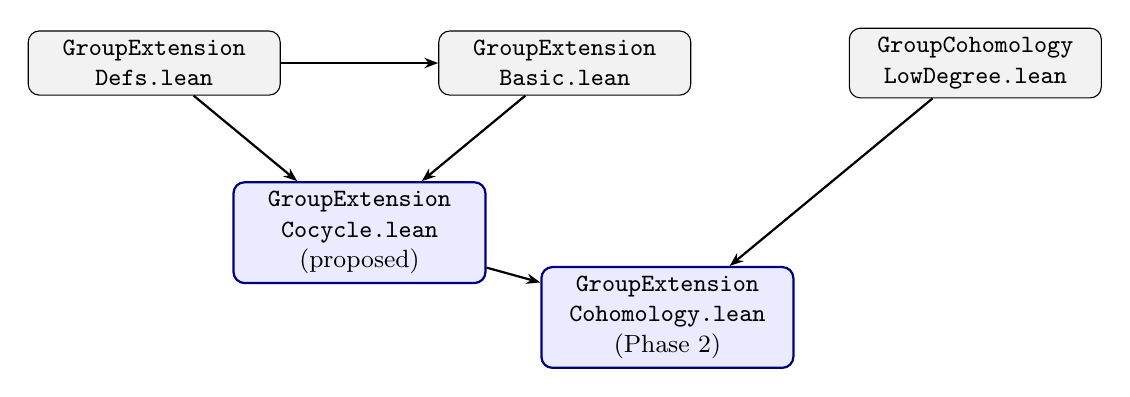
\begin{tikzpicture}[
  box/.style={draw, rounded corners, minimum width=3.2cm, minimum height=0.8cm,
              align=center, font=\small},
  newbox/.style={box, fill=blue!8, draw=blue!50!black, thick},
  oldbox/.style={box, fill=gray!10},
  arr/.style={-{Stealth[length=5pt]}, thick},
  node distance=1.2cm and 1.5cm
]
  \node[oldbox] (defs) {\texttt{GroupExtension}\\\texttt{Defs.lean}};
  \node[oldbox, right=2cm of defs] (basic) {\texttt{GroupExtension}\\\texttt{Basic.lean}};
  \node[newbox, below=1.5cm of $(defs)!0.5!(basic)$] (cocycle)
    {\texttt{GroupExtension}\\\texttt{Cocycle.lean}\\(proposed)};
  \node[oldbox, right=2cm of basic] (lowdeg) {\texttt{GroupCohomology}\\\texttt{LowDegree.lean}};
  \node[newbox, below=1.5cm of $(cocycle)!0.5!(lowdeg)$] (bridge)
    {\texttt{GroupExtension}\\\texttt{Cohomology.lean}\\(Phase 2)};

  \draw[arr] (defs) -- (basic);
  \draw[arr] (defs) -- (cocycle);
  \draw[arr] (basic) -- (cocycle);
  \draw[arr] (cocycle) -- (bridge);
  \draw[arr] (lowdeg) -- (bridge);
\end{tikzpicture}
\end{center}

%=======================================================================
\section{Dependency Structure and Proof Architecture}\label{sec:deps}
%=======================================================================

The internal dependency structure of our proposed theorems is shown below. An arrow
$A \to B$ means $B$ depends on $A$ in its proof.

\begin{center}
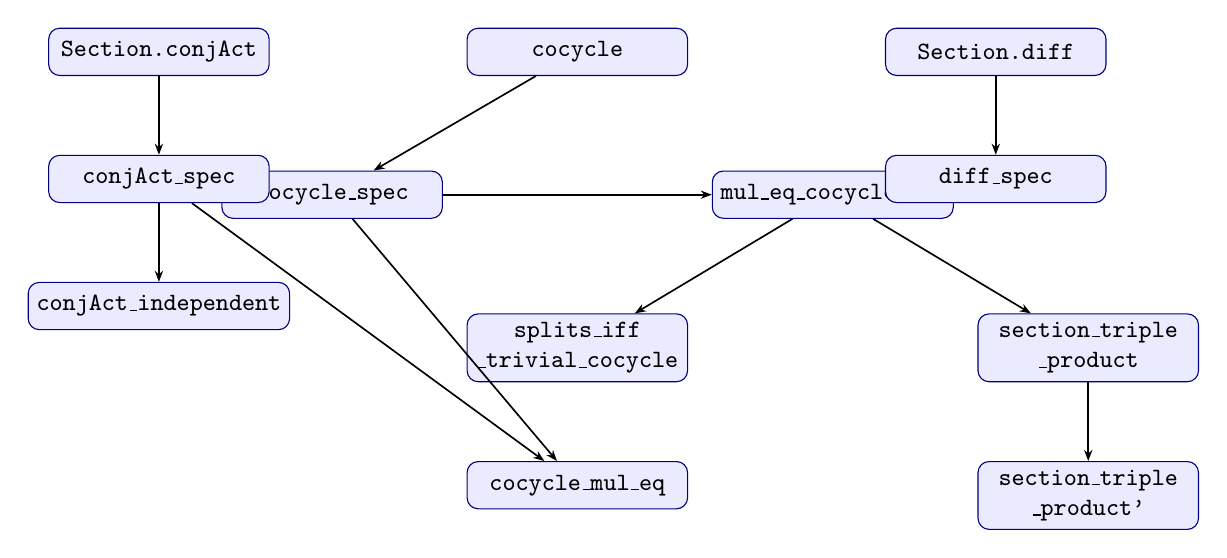
\begin{tikzpicture}[
  node distance=1.0cm and 2.2cm,
  every node/.style={draw, rounded corners, font=\small\ttfamily, minimum width=2.8cm,
                     minimum height=0.6cm, align=center, inner sep=3pt},
  new/.style={fill=blue!8, draw=blue!50!black},
  arr/.style={-{Stealth[length=4pt]}, semithick}
]
  \node[new] (defect) {cocycle};
  \node[new, below left=1.2cm and 0.3cm of defect] (spec) {cocycle\_spec};
  \node[new, below right=1.2cm and 0.3cm of defect] (muleq) {mul\_eq\_cocycle\_mul};
  \node[new, below left=1.2cm and 0.3cm of muleq] (splits) {splits\_iff\\\_trivial\_cocycle};
  \node[new, below right=1.2cm and 0.3cm of muleq] (triple) {section\_triple\\\_product};
  \node[new, below=1.0cm of triple] (triple2) {section\_triple\\\_product'};

  \node[new, right=2.5cm of defect] (diff) {Section.diff};
  \node[new, below=1.0cm of diff] (diffspec) {diff\_spec};

  \node[new, left=2.5cm of defect] (conjact) {Section.conjAct};
  \node[new, below=1.0cm of conjact] (conjspec) {conjAct\_spec};
  \node[new, below=1.0cm of conjspec] (conjind) {conjAct\_independent};

  \node[new, below=1.0cm of splits] (cocid) {cocycle\_mul\_eq};

  \draw[arr] (defect) -- (spec);
  \draw[arr] (spec) -- (muleq);
  \draw[arr] (muleq) -- (splits);
  \draw[arr] (muleq) -- (triple);
  \draw[arr] (triple) -- (triple2);
  \draw[arr] (spec) -- (cocid);
  \draw[arr] (conjspec) -- (cocid);

  \draw[arr] (diff) -- (diffspec);

  \draw[arr] (conjact) -- (conjspec);
  \draw[arr] (conjspec) -- (conjind);
\end{tikzpicture}
\end{center}

\subsection{Proof strategy overview}

The proofs follow a uniform strategy:

\begin{enumerate}[nosep]
\item \textbf{Membership lemma}: Reuse the existing Mathlib lemma
  (\texttt{mul\_mul\_mul\_inv\_mem\_range\_inl} or \texttt{mul\_inv\_mem\_range\_inl})
  establishing that the relevant expression lies in
  $\mathrm{range}(\texttt{inl}) = \ker(\texttt{rightHom})$.

\item \textbf{Definition via \texttt{choose}}: Extract the $N$-valued preimage using
  \texttt{Exists.choose} on the membership proof.

\item \textbf{Specification via \texttt{choose\_spec}}: The specification lemma
  (\texttt{cocycle\_spec}, \texttt{diff\_spec}) is simply \texttt{Exists.choose\_spec}.

\item \textbf{Downstream theorems via injectivity}: All equalities between $N$-valued
  expressions are proved by applying \texttt{S.inl\_injective} and then rewriting
  using the specification lemmas. This reduces $N$-level reasoning to $E$-level
  group algebra.
\end{enumerate}

This ``push through \texttt{inl}, reason in $E$, pull back via injectivity'' pattern
is the key proof engineering technique. It avoids working directly with the
noncomputable \texttt{choose} and instead works entirely through the specification
interface.

%=======================================================================
\section{\texorpdfstring{Toward $H^1$ and $H^2$: Phase~2 Roadmap}{Toward H1 and H2: Phase 2 Roadmap}}\label{sec:roadmap}
%=======================================================================

\subsection{\texorpdfstring{Phase~2a: The $H^1$ bridge}{Phase 2a: The H1 bridge}}

\textbf{Target theorem:}
\[
  \texttt{GroupExtension.ConjClasses} \;\simeq\; H^1(G, N)
  \qquad\text{(for abelian $N$, split extension)}
\]

\textbf{What we provide (Phase~1):}
\begin{itemize}[nosep]
\item \texttt{Section.conjAct}: The $G$-action on $N$ via sections.
\item \texttt{Section.conjAct\_independent}: For abelian $N$, the action is
  section-independent (so it descends to a well-defined $G$-module structure).
\item \texttt{Section.diff}: The difference function between sections.
\end{itemize}

\textbf{What remains (Phase~2):}
\begin{itemize}[nosep]
\item Show that the difference function between two splittings is a 1-cocycle.
\item Show that $N$-conjugation changes the splitting by a 1-coboundary.
\item Construct the bijection between \texttt{ConjClasses} and $H^1$.
\end{itemize}

\subsection{\texorpdfstring{Phase~2b: The $H^2$ bridge}{Phase 2b: The H2 bridge}}

\textbf{Target theorem:}
\[
  \{\text{equivalence classes of extensions with kernel $N$ and action $\varphi$}\}
  \;\simeq\; H^2(G, N)
\]

\textbf{What we provide (Phase~1):}
\begin{itemize}[nosep]
\item \texttt{Section.cocycle}: The $N$-valued 2-cocycle.
\item \texttt{Section.cocycle\_mul\_eq}: The 2-cocycle identity.
\item \texttt{Section.diff}: The section difference function.
\item \texttt{splits\_iff\_trivial\_cocycle}: Splitting iff trivial cocycle class.
\end{itemize}

\textbf{What remains (Phase~2):}
\begin{itemize}[nosep]
\item \textbf{Cocycle change formula}: For sections $\sigma, \sigma'$ with difference
  $d = \mathrm{diff}(\sigma, \sigma')$, prove
  \[
    c_{\sigma'}(g_1, g_2) = d(g_1) \cdot \varphi(g_1)(d(g_2)) \cdot c_\sigma(g_1, g_2)
    \cdot d(g_1 g_2)^{-1}
  \]
  showing the cocycles differ by a coboundary.

\item \textbf{Type-theoretic bridge}: For abelian $N$, coerce the
  multiplicative cocycle into the setting required by Mathlib's
  \texttt{Rep k G}-based \texttt{H2}. This involves:
  (i)~uncurrying via \texttt{Function.uncurry},
  (ii)~extracting a \texttt{MulDistribMulAction} from the \texttt{MulAut}-valued
  conjugation action, and
  (iii)~applying \texttt{cocyclesOfIsMulCocycle\textsubscript{2}} to obtain an element
  of \texttt{cocycles\textsubscript{2}}.

\item \textbf{Extension equivalence}: Define equivalence of extensions (with fixed
  kernel and quotient) and construct the bijection with $H^2$.
\end{itemize}

\subsection{Estimated effort}

\begin{center}
\begin{tabular}{lll}
\toprule
\textbf{Phase} & \textbf{Scope} & \textbf{Status} \\
\midrule
Phase 1 (this PR) & Cocycle + splitting criterion & Complete (zero sorry) \\
Phase 2a ($H^1$) & Conjugacy classes $\leftrightarrow$ $H^1$ & Future work \\
Phase 2b ($H^2$) & Extension classes $\leftrightarrow$ $H^2$ & Future work \\
\bottomrule
\end{tabular}
\end{center}

The main bottleneck for Phase~2b is the type-theoretic bridge between multiplicative
$N$-valued cocycles and Mathlib's $k$-linear representation-theoretic $H^2$. If this
bridge proves too heavy, a fallback is to define a multiplicative $H^2_{\mathrm{mul}}$
directly (as the quotient of multiplicative 2-cocycles by multiplicative 2-coboundaries)
and prove the classification theorem in that setting, deferring the connection to
Mathlib's \texttt{groupCohomology.H2} to a subsequent PR.

%=======================================================================
\section{Testing and Compatibility}\label{sec:testing}
%=======================================================================

\subsection{Build status}

The development builds successfully against Mathlib v4.29.0-rc6 (Lean~4 toolchain
\texttt{leanprover/lean4:v4.29.0-rc6}). All files compile with \texttt{lake build}
with no errors and zero \texttt{sorry}.

\subsection{Proof status}\label{sec:sorry}

All theorems in the development are \textbf{fully verified} by the Lean type checker
with \textbf{zero \texttt{sorry}}. In particular, the 2-cocycle identity
(\texttt{Section.cocycle\_mul\_eq}) is completely proved.

The proof proceeds by applying \texttt{S.inl\_injective} to reduce the $N$-level
equality to an $E$-level equality, then uses a pair of auxiliary \texttt{have} lemmas
(\texttt{lhs} and \texttt{rhs}) that each simplify one side via
\texttt{section\_mul\_eq} rewrites and associativity/cancellation steps. The final step
applies \texttt{mul\_right\_cancel} to equate the two sides.

\begin{lstlisting}
theorem sectionCocycle_isMulCocycle₂_conj
    (σ : S.Section) (g₁ g₂ g₃ : G) :
    sectionCocycle S σ g₁ g₂ *
      sectionCocycle S σ (g₁ * g₂) g₃ =
    sectionConjAct S σ g₁
      (sectionCocycle S σ g₂ g₃) *
      sectionCocycle S σ g₁ (g₂ * g₃) := by
  apply S.inl_injective
  rw [map_mul, map_mul, inl_sectionConjAct]
  have lhs : ... := by
    rw [mul_assoc, ← section_mul_eq S σ (g₁ * g₂) g₃,
        ← mul_assoc, ← section_mul_eq S σ g₁ g₂]
  have rhs : ... := by
    rw [mul_assoc _ (S.inl ...)]
    rw [← section_mul_eq S σ g₁ (g₂ * g₃)]
    rw [mul_assoc _ (σ.toFun g₁)⁻¹, inv_mul_cancel_left]
    rw [mul_assoc, ← section_mul_eq S σ g₂ g₃,
        ← mul_assoc]
  apply mul_right_cancel
    (b := σ.toFun (g₁ * g₂ * g₃))
  rw [lhs, show g₁ * g₂ * g₃ = g₁ * (g₂ * g₃)
        from mul_assoc g₁ g₂ g₃, rhs]
\end{lstlisting}

\textbf{Note on factor order.} The correct statement places $c(g_1, g_2)$ before
$c(g_1 g_2, g_3)$ on the left-hand side. An earlier draft had the factors reversed;
correcting the order was the key step that enabled the proof to close.

\subsection{Module structure}

The proposed Mathlib file \texttt{Mathlib/GroupTheory/GroupExtension/Cocycle.lean}
would contain all definitions and theorems from \Cref{tab:api-defs,tab:api-thms}.
The file structure follows Mathlib conventions:

\begin{lstlisting}
/-
  GroupExtension.Cocycle -- Section cocycles and
  splitting criteria for group extensions.

  ## Main definitions

  * `GroupExtension.Section.cocycle`
  * `GroupExtension.Section.diff`
  * `GroupExtension.Section.conjAct`

  ## Main results

  * `GroupExtension.splits_iff_trivial_cocycle`
  * `GroupExtension.Section.cocycle_spec`
  * `GroupExtension.Section.cocycle_mul_eq`

  ## References

  See the TODO in `GroupExtension/Defs.lean` (lines 43-52).
  This module is Phase 1 toward completing the H1/H2
  classification theorems documented there.
-/

import Mathlib.GroupTheory.GroupExtension.Basic
\end{lstlisting}

\subsection{Interaction with existing \texttt{simp} lemmas}

We have verified that our proposed \texttt{@[simp]} lemmas do not conflict with
existing Mathlib \texttt{simp} lemmas for \texttt{GroupExtension}. The key observation
is that our \texttt{simp} lemmas rewrite \texttt{S.inl (cocycle ...)} and
\texttt{S.inl (diff ...)}, which are new term patterns not matched by any existing
\texttt{simp} lemma. There is no risk of \texttt{simp} loops.

\subsection{AI use disclosure}

Per Mathlib's policy on AI-assisted contributions, the PR description will disclose
that AI tools (Claude) were used in the development of this contribution, including
proof exploration, tactic suggestion, and documentation drafting. All mathematical
content has been verified by the Lean type checker with zero \texttt{sorry}.

%=======================================================================
% Bibliography
%=======================================================================

\begin{thebibliography}{5}

\bibitem{brown}
K.\,S.~Brown,
\emph{Cohomology of Groups},
Graduate Texts in Mathematics, vol.~87,
Springer-Verlag, 1982.
\newblock \url{https://doi.org/10.1007/978-1-4684-9327-6}

\bibitem{mathlib-groupext}
Mathlib Contributors,
\emph{Mathlib.GroupTheory.GroupExtension.Defs},
2024--2026.
\newblock \url{https://leanprover-community.github.io/mathlib4_docs/Mathlib/GroupTheory/GroupExtension/Defs.html}

\bibitem{mathlib-groupext-basic}
Mathlib Contributors,
\emph{Mathlib.GroupTheory.GroupExtension.Basic},
2024--2026.
\newblock \url{https://leanprover-community.github.io/mathlib4_docs/Mathlib/GroupTheory/GroupExtension/Basic.html}

\bibitem{mathlib-lowdegree}
Mathlib Contributors,
\emph{Mathlib.RepresentationTheory.Homological.GroupCohomology.LowDegree},
2024--2026.
\newblock \url{https://leanprover-community.github.io/mathlib4_docs/Mathlib/RepresentationTheory/Homological/GroupCohomology/LowDegree.html}

\bibitem{lean4}
L.~de~Moura and S.~Ullrich,
``The Lean~4 theorem prover and programming language,''
in \emph{Automated Deduction -- CADE 28}, LNCS, vol.~12699,
Springer, 2021, pp.~625--635.

\end{thebibliography}

\end{document}
